\begin{frame}{Contribution 1: Survey}
    \begin{block}{Objective}
        We first provide a comprehensive review of the literature through a survey.
    \end{block}
\end{frame}

\begin{frame}{Contribution 1: Survey}{Methodology}
    \begin{columns}
        \column{0.5\textwidth}
        Search Engines (3)
        \begin{itemize}
            \item Google Scholar
            \item PubMed's search engine
            \item Sofia
        \end{itemize}

        \column{0.5\textwidth}
        Keywords (19)
        \begin{itemize}
            \item machine learning
            \item deep learning
            \item ABP
            \item estimation
            \item PPG
            \item continuous
            \item non-invasive
            \item cuffless
            \item etc.
        \end{itemize}
    \end{columns}

    \pause
    \vspace{1cm}
    \centering
    \alert{50 articles, 176 models}
\end{frame}

\begin{frame}{Contribution 1: Survey}{Methodology}
    \begin{itemize}
        \item Dataset
        \item Preprocessing
        \item Model architecture
        \item Performance
    \end{itemize}
    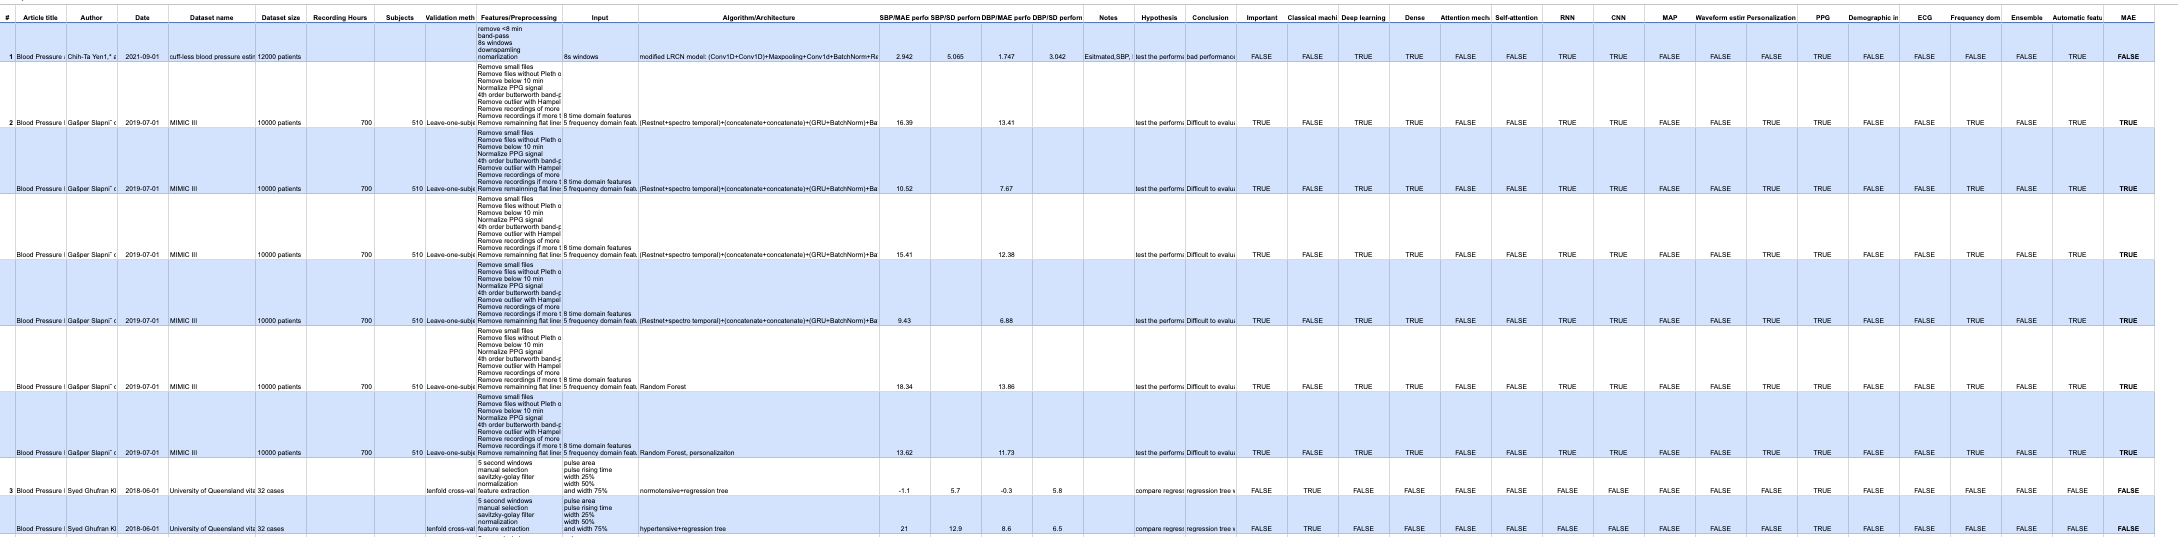
\includegraphics[width=\textwidth]{survey/bigtable.png}
    \href{https://docs.google.com/spreadsheets/u/1/d/e/2PACX-1vR-3MoAcaD-N30ZM15ozSlxh8RHTUBv2KETb9f2g852htlH-5PNt_S8khVnUFLWeEo2H91ZW9hCEi8o/pubhtml}{published online for viewing}
\end{frame}

\begin{frame}{Contribution 1: Survey}{Results}
    \centering
    \includesvg[scale=0.6]{survey/Taxonomy.drawio.svg}
\end{frame}

\begin{frame}{Contribution 1: Survey}{Results}
    Methods
    \begin{figure}
        \includesvg[width=0.3\columnwidth]{survey/layers.svg}
        \hfill
        \includesvg[width=0.3\columnwidth]{survey/input.svg}
        \hfill
        \includesvg[width=0.3\columnwidth]{survey/algorithm.svg}
    \end{figure}
    \begin{itemize}
        \item PPG
        \item Deep Learning
        \item Dense, RNN, CNN
    \end{itemize}
\end{frame}

\begin{frame}{Contribution 1: Survey}{Results}
    Years
    \begin{columns}
        \column{0.7\columnwidth}
        \begin{figure}
            \includesvg[width=\columnwidth]{survey/years.svg}
        \end{figure}

        \column{0.3\columnwidth}
        \begin{itemize}
            \item Almost all after 2018
        \end{itemize}
    \end{columns}


\end{frame}

\begin{frame}{Contribution 1: Survey}{Results}
    Reported Performance

    \begin{figure}
        \includesvg[width=0.49\columnwidth]{survey/mae.svg}
        \includesvg[width=0.49\columnwidth]{survey/sd.svg}
    \end{figure}

    \begin{itemize}
        \item 36 SBP
        \item 54 DBP
        \item 36 SBP \& DBP, $32\%$
    \end{itemize}
\end{frame}

\begin{frame}{Contribution 1: Survey}{Results}
    Filter articles based on annotations
    \begin{itemize}
        \item PPG Only
        \item Automatic Feature Extraction
        \item Public datasets only
        \item MAE performance metric
    \end{itemize}

    \pause
    \alert{8 articles, 9 models}
\end{frame}

\begin{frame}{Contribution 1: Survey}{Results}
    \begin{table}
        \centering
        \tiny
        \begin{tabularx}{\textwidth}{ l >{\raggedright\arraybackslash}X l >{\raggedright\arraybackslash}X }
            \hline
            No. & \thead{Authors}                                 & \thead{Architecture}                                             \\
            \hline
            1   & Slapničar et al. \cite{slapnicar_blood_2019}    & spectro-temporal ResNet inspired                                 \\
            2   & Athaya and Choi \cite{athaya_estimation_2021}   & U-Net inspired                                                   \\
            3   & Chen et al. \cite{chen_new_2022}                & RSPAN                                                            \\
            4   & Harfiya et al. \cite{harfiya_continuous_2021}   & LSTM autoencoder                                                 \\
            5   & Kim et al. \cite{kim_deepcnap_2022}             & ResUNet with attention-based skip connections and self-attention \\
            6   & Leitner et al. \cite{leitner_personalized_2022} & CNN, GRU, Dense                                                  \\
            7   & Tazarv and Levorato \cite{tazarv_deep_2021}     & CNN, LSTM, Dense                                                 \\
            8   & Schrumpf et al. \cite{schrumpf_assessment_2021} & AlexNet                                                          \\
            9   & Schrumpf et al. \cite{schrumpf_assessment_2021} & ResNet                                                           \\
            \hline
        \end{tabularx}
    \end{table}
    \begin{table}
        \centering
        \tiny
        \begin{tabularx}{\textwidth}{ l X r  r }
            \hline
            Authors                                         & \thead{Validation Method}                   & \thead{Subjects} & \thead{Recording Hours} \\
            \hline
            Slapničar et al. \cite{slapnicar_blood_2019}    & Leave-one-subject-out                       & 510              & 700                     \\
            Athaya and Choi \cite{athaya_estimation_2021}   & 70/15/15                                    & 100              & 195                     \\
            Chen et al. \cite{chen_new_2022}                & 10-fold cross-validation                    & 1562             & -                       \\
            Harfiya et al. \cite{harfiya_continuous_2021}   & 70/10/20                                    & 5289             & -                       \\
            Kim et al. \cite{kim_deepcnap_2022}             & 10-fold cross-validation                    & 2064             & 374.43                  \\
            Leitner et al. \cite{leitner_personalized_2022} & 5-fold cross-validation per subject         & 100              & 1000                    \\
            Tazarv and Levorato \cite{tazarv_deep_2021}     & Leave-one-window-out, one model per patient & 20               & 1.66                    \\
            Schrumpf et al. \cite{schrumpf_assessment_2021} & 75/12.5/12.5, patient-wise                  & 5000             & -                       \\
            \hline
        \end{tabularx}
    \end{table}
\end{frame}